\chapter{Reinforcement Learning}
\begin{quotation}
\noindent ``\emph{quote}''
\begin{flushright}\textbf{auteur, date}\end{flushright}
\end{quotation}

\vspace*{0.5cm}


\section{The reinforcement learning problem}
A reinforcement learning setting sees two main components interact : the agent
(an entity performing actions)
and the environment. The environment can be in several states which the agent
can observe (for example in the CartPole problem : the cart can be in several 
positions and have different velocities, and the pole has similar 
characteristics). In some problems, the agent might not be able to observe the
full state of the environment.\\

The agent chooses actions based on its knowledge of the state of the
environment. These actions might (and often do) alter the state of the
environment, but will also generate a reward. In the CartPole problem, the 
reward is +1 every tick the pole is above a certain angle, 0 otherwise. The
goal of the agent is to maximise the obtained reward.\\

With this simple setting, of which a diagram is shown in Figure~\ref{fig:rl},
we can design algorithms that can be trained to solve a huge variety of tasks
without ever having to include task-specific logic to the algorithm.

\begin{figure}[]
	\centering
	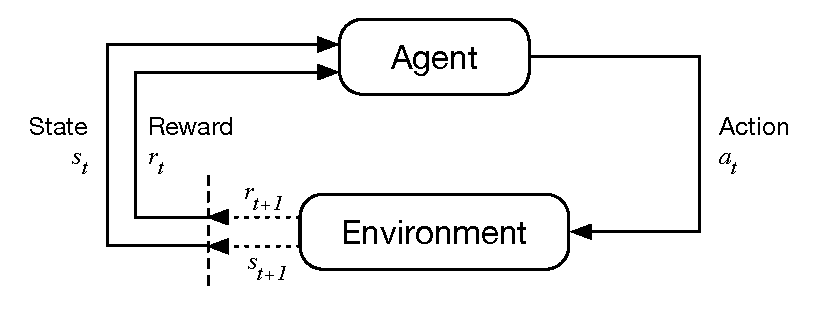
\includegraphics[width=0.65\linewidth]{fig/rl.eps}
	\caption{The setting of a reinforcement learning problem 
		\cite{suttonbarto}}
	\label{fig:rl}
\end{figure}

\subsection{Markov Decision Processes}
A reinforcement learning problem can be formally defined as a Markov 
Decision Process (MDP) \index{MDP} characterised by :
\begin{itemize}
	\item a set of states $\mathcal{S}$
	\item a set of actions $\mathcal{A}$
	\item a transition function 
		$T(s, a, s') = P(s_{t+1} = s' \mid s_t = s, a_t = a)$
	\item a reward function 
		$r(s, a, s') = \mathbb{E}
		 [r_{t+1} \mid s_t = s, a_t = a, s_{t+1} = s']$
\end{itemize}
For the rest of this paper, we will consider that the transition function is
deterministic.\\

The goal of reinforcement learning is for the agent to select, in any state it
can be in, the action that will lead it to the highest expected reward :

\begin{equation}
\label{eq:discounted_reward}
R_t = \mathbb{E}[r] = r_t + \gamma r_{t+1} + \gamma^2 r_{t+2}^2 + ... =
 \sum\limits_{i=0}^\infty \gamma^i r_{t+i}
\end{equation}

\noindent with the discount factor \index{discount factor} $\gamma \in [0, 1[$.
The discount factor allows one to tune the agent's behaviour on the
short-term/long-term spectrum. A discount factor $\gamma=0$ would mean that the
agent maximises its expected reward for the next transition only whereas a
discount factor close to one will favour behaviour that maximises long-term
reward, even if one action leads to a poor reward at first.\\

\subsection{Policy}
\index{policy}
The agent uses a policy $\pi(a \mid s)$ which describes a probability
distribution over the action set $\mathcal{A}$, determining the probability of
selecting action each action $a_i in \mathcal{A}$ once it is
in a certain state $s_i$. This policy is \textbf{deterministic} if and only if:
\begin{equation}
\forall\, s \in \mathcal{S},\; \exists\, a \in \mathcal{A} : \pi(a \mid s) = 1
\end{equation}
\noindent In other words : in any state, only one action can be selected.
Otherwise, the policy is \textbf{stochastic}.

\section{An example : the 2-armed bandit problem}
The 2-armed bandit setting defines two actions that the agent can perform,
each of which associated with one arm. Each arm has an underlying reward
distribution -- for the sake of this example, let us define each arm with the
following Bernoulli distributions: \index{Bernoulli}

\begin{table}[H]
	\centering
	\begin{tabular}{c|c}
		Arm \#1 & Arm \#2 \\ \hline
		0.9 & 0.1
	\end{tabular}
\end{table}

\noindent This means that arm \#1 will generate a reward of 1 with a probability
of 0.9 and arm \#2 will generate a reward of 1 with a probability of 0.1.\\

The careful reader will have noticed that this problem is stateless 
($\mathcal{S} = \{\varnothing\}$), meaning that the agent only perceives
rewards and no state observations.\\

Of course, before its first interaction with the environment, the agent has no
information whatsoever about the reward distribution of each arm, and the whole
idea of reinforcement learning is to look for evermore efficient ways to learn
the structure and parameters of a problem in order to maximise reward.\\

One could imagine a simple strategy like the following : play each arm 10 times,
then always play the arm with the highest average reward. This policy is
deterministic, and yields either $ \pi(a_1) = 1$ and $\pi(a_2) = 0$ or
$\pi(a_1) = 0$ and $\pi(a_2) = 1$. This could work in
our case, but might fail in cases where the distributions are much closer
(e.g. 0.45 and 0.55). What if the reward was sampled out of overlapping normal
distributions?\\

Deciding whether the following action should be used to explore the environment
and gain information about it; or to exploit the information already available
to try to maximise reward is not trivial. Exploring could make training slower
or affect the reward if our model of the environment is correct, but it is 
needed to increase the probability that we have indeed a correct model. This
tradeoff is called the exploration/exploitation tradeoff. \index{exploration}
\index{exploitation}


\section{Neural networks for reinforcement learning}
As hinted at previously, neural networks are powerful function approximators and
have yielded impressive results in reinforcement learning. They are used either
directly as policy functions, taking a state as input and outputting a
probability distribution over the action set; or as value estimators, by 
outputting a scalar which estimates the value of states and actions related to the
estimated achievable discounted reward from those states.

\subsection{Policy gradient methods}
Policy gradient methods are rather straightforward ways of learning to solve a task.
Let us assume that the
policy is defined by a neural network of which the input layer is set to 
receive an observation of the state of the environment and the output layer
defines a policy (a probability distribution over the actions set).
Training starts with a randomly initialised policy. 
When the agent performs an action chosen with its policy, the environment will
update its state and the agent will receive an observation of this state as
well as a reward signal. We can use the reward signal to proportionately
encourage (if the reward is 
positive) or discourage (if the reward is negative) taking this action in 
this specific state.\\

As the policy is defined by a neural network, we have to define a way to
update the network to find the best policy. This is done by defining a loss
function of which the gradient will be propagated back into the network, or
by defining directly the gradient as a parameters update rule.\\

Let us suppose that the agent is in a situation where it can perform two
actions, and it has received a reward of +5 after choosing action 2
sampled out of its policy $\pi(s) = [0.1, 0.9]$. We can directly use the
reward signal as a gradient to update the network. Indeed, setting gradients
to $[0, 5]$ (because a +5 reward was generated by action 2) and multiplying it 
to the gradient of the policy $\nabla \pi(a \mid s)$ will make the network
learn what actions to perform under certain states by directly increasing the
probability of playing actions which receive a positive reward, and by
decreasing the probability of actions which receive a negative reward.\\

The method as presented still presents an issue in the sense that it only takes
into account immediate reward, but we may want to maximise long-term reward.
Let $R_t$, the discounted future reward at time step $t$ (see equation 
\ref{eq:discounted_reward}), be the metric
that we want to maximise. In a policy gradients method, we will update the
neural network policy directly with :
\begin{equation}
	\label{eq:policy_update_rule}
	\alpha \nabla \pi(a \mid s) R_t
\end{equation}
in which $\alpha$ is the learning rate and $a$ was the chosen action.

\subsection{Value methods}
There is another category of methods which use an estimate of the value of
actions or states; in other words functions which map states or state-action
pairs to estimates of their discounted future reward $R_t$. Once again, we can
use neural networks to estimate such functions. We then only have to define
a policy that decides which actions to take given these value estimates; one
example of such a policy could be a deterministic policy choosing the action
leading to the state with the highest value.\\

\paragraph{V-values} estimate the value of a state; i.e. the estimated
discounted reward achievable from a specific state.
The optimal state value function 
$$ V^*(s) = R_t = \mathbb{E}
   \left[ r_t + \gamma r_{t+1} + \gamma^2 r_{t+2}^2 + ...  \right]$$
can be estimated using a Bellman equation in the following way :
$$ V(s) = \mathbb{E}\left[ r_t + \gamma V(s')\right]$$
where $s'$ is the state reached after $s$.\\

Indeed, under the condition that $V(s)$ is optimal, the value of a state is the 
sum of the discounted value of the unique optimal next state and the reward of
the transition to that next state.\\

This can be used as an update rule for the $V$ network with a loss similar to :
\begin{equation}
	\label{eq:v_update_rule}
\left[V(s) -  \left(r_t + \gamma V(s') \right)\right]^2 
\end{equation}
\noindent which is a simple mean squared error between the estimation $V(s)$ and
the target $\left(r_t + \gamma V(s') \right)$.

\paragraph{Q-values} estimate the value of state-action pairs; i.e. the
estimated discounted reward achievable when taking a specific action in a 
specific state. The reasoning to find an update rule is similar for V-values
and Q-values. The optimal Q function can be estimated with a Bellman equation :
$$ Q(s, a) = \mathbb{E}\left[ r_t + \gamma \max\limits_{a'} Q(s', a') \right]$$
\noindent and so can be deduced an update rule for Q networks of which the loss
can be defined with the following :

\begin{equation}
	\label{eq:q_update_rule}
\left[Q(s, a) - \left( r_t + \gamma \max\limits_{a'} Q(s', a') \right) \right]^2
\end{equation}


\subsection{Actor-Critic}
Value methods present the issue of having to manually decide on a policy.
Actor-critic methods have both an \textit{actor} (the policy) and a
\textit{critic} (value functions). The actor performs the actions, and the 
critic updates the policy. One way to update the policy using a critic is to
scale the policy gradient using our current estimate of the V function:
\begin{equation}
	\label{eq:adv_update_rule}
\nabla \pi(a_t \mid s_t) (R_t - V(s_t))
\end{equation}
This way, the policy will be updated according to how wrong the critic was.
The value $R_t - V(s_t)$ is called the \textbf{advantage} \index{advantage}
because it expresses how much better (or worse) the reward was compared to 
what was estimated.


\subsubsection{The A2C algorithm}
We now have all the cards in our hand to understand the A2C
(Advantage Actor-Critic) algorithm which is a simpler version of A3C \cite{a3c}
(it only uses one thread instead of being asynchronous). 
A2C consists of a neural network
of which the input is the state $s_t$, and which outputs both a value function
$V(s_t)$ and a policy $\pi(s_t)$ (see Figure~\ref{fig:a2c}). These outputs
respectively use the updates rules described in equations \ref{eq:v_update_rule}
and \ref{eq:adv_update_rule}.  Algorithm~\ref{algo:a2c} shows the training
process of the A2C agent which alternates playing episodes and updating the
network according to the agent's experience.

\begin{figure}[]
	\centering
	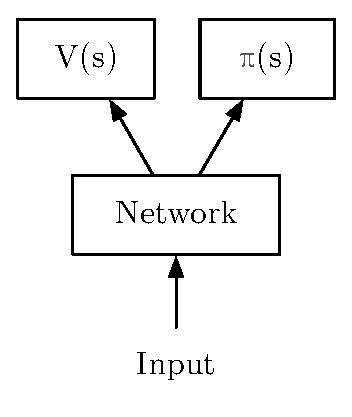
\includegraphics[width=0.2\linewidth]{fig/a3c.eps}
	\caption{The A2C network}
	\label{fig:a2c}
\end{figure}

\begin{algorithm}
\caption{The A2C training process}
\label{algo:a2c}
\begin{algorithmic}[1]
\State{$T_{\text{max}} \leftarrow$ maximum number of ticks}
\While{$T < T_{\text{max}}$}
	\Statex
	\State{\textit{// Play an episode}}
	\State{$t \leftarrow 0$}
	\While{$t <$ maximum episode length \textbf{or} episode not finished}
		\State{perform $a_t$ sampled using $\pi(s_t)$}
		\State{record reward $r_t$ and new state $s_{t+1}$}
		\State{$t \leftarrow t+1$}
	\EndWhile
	\State{$T \leftarrow T + t$}
	\Statex
	\State{\textit{// Compute advantages and gradients by unrolling episode}}
	\State{$d\theta_p \leftarrow 0$ \textit{// policy gradient}}
	\State{$d\theta_v \leftarrow 0$ \textit{// value gradient}}
	\For{$i \in \{t-1,\; t-2,\; ...,\; 0\}$}
		\State{$R \leftarrow r_i + \gamma R$}
		\State{$d\theta_p \leftarrow d\theta_p + \nabla \pi(a_i|s_i)(R-V(s_i))$}
		\State{$d\theta_v \leftarrow d\theta_v + \nabla (R - V(s_i))^2$}
	\EndFor
	\State{Update policy network using $d\theta_p$}
	\State{Update value network using $d\theta_v$}
	\Statex
\EndWhile

\end{algorithmic}
\end{algorithm}


